\chapter{Análisis Comparativo}
Android e iOS son dos plataformas muy populares entre los dispositivos móviles. Es por ello, que existes muchas  muchas formas de comparar sus respectivos módulos de seguridad.\\

La medida de comparación propuesta en \cite{YA2014} consiste en analizar la seguridad de una aplicación móvil en cada fase del ciclo de vida, comparándola en cada plataforma.\\

En \cite{HYGZD13} el enfoque es distinto. Se centra en comparar los permisos requeridos a cada plataforma al momento de instalar aplicaciones presentes en ambas plataformas.\\

En \cite{Gor16, BCLR15, Rom14} se cambia el enfoque propuesto. El objetivo que persiguen es desarrollar una especificación formal que describa el modulo de seguridad de Android.\\

En cambio, en \cite{TZSH13}, el enfoque se centra en distintos ataques al modelo de seguridad de iOS.\\

En este capítulo se propone una forma de comparar distinta a las anteriores. Consiste en analizar distintas características presentes en ambas plataformas, poniendo foco en los permisos que se pueden modificar \emph{en tiempo de ejecución}. El análisis se esta basado en los documentos oficiales de seguridad, tales como \cite{aossec, asreview2015, asg} entre otros. Al final del capítulo se agrega una crítica sobre las funcionalidades mencionadas en el análisis.
\section{Analizando Android}
\subsection{Autenticación del usuario}
Android provee diversas formas para que un usuario se autentique, con el objetivo de desbloquear la pantalla. Desde los comienzos, la autenticación se realizaba mediante el PIN, contraseña y patrones. A partir de la versión 5.0, se introduce el concepto llamado \textit{TrustAgents}, el cuál permite mecanismos de desbloqueo más flexibles, tales como:
\begin{itemize}
	\item Reconocimiento facial.
	\item Un determinado lugar, configurado a través de Google Maps.
	\item Reconocimiento de voz.
	\item Ciertos dispositivos, tales como el auto (a través de Bluetooth).
\end{itemize}
La novedad en la versión 6.0 es que soporta el lector de huellas digitales.\\

Dependiendo del método utilizado para autenticarse, el sistema operativo provee dos componentes: \textit{Gatekeeper} y \textit{Fingerprint}. El primer componente realiza la autenticación del patrón/contraseña del dispositivo en un entorno de ejecución de confianza TEE\footnote{El \textit{Trust Execution Enviroment} es una zona segura del procesador principal en la cual se provee una ejecución segura e íntegra, tanto de código fuente como de datos. El TEE aisla por \textit{hardware} el acceso a cierta memoria y provee mecanismos de I/O para dicha memoria \cite{tee2011}.}; mientras que el segundo componente es el encargado de verificar que la huella detectada por el sensor es valida. Ellos interactúan con el \textit{Keystore}\footnote{Es un componente para almacenar las claves criptográficas, el cual dificulta su extracción, ya que asegura dos cosas: una clave nunca entra en una aplicación y una clave nunca sale de una zona segura \cite{dakss}.} para soportar el uso de \textit{tokens} de autenticación respaldados por \textit{hardware} (\textit{AuthTokens}).\\

La verificación del desbloqueo de la pantalla ocurre en el TEE, tal como se observa en la Figura \ref{fig:ch01:authentication-flow}.\\

\begin{figure}[htbp]
	\begin{center}
		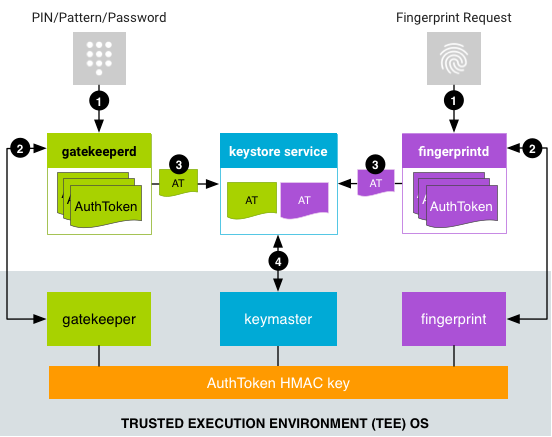
\includegraphics[width=0.7\linewidth]{chapter1/authentication-flow}
		\caption{Proceso de autenticación en Android\cite{aossec}.}
		\label{fig:ch01:authentication-flow}
	\end{center}
\end{figure}
Como consecuencia del esta forma de autenticarse, se destacan las siguientes ventajas:
\begin{itemize}
    \item Al permitir el desbloqueo con datos biométricos, se acelera y se simplifica el proceso de autenticación. Los usuarios eligen este sistema de desbloqueo en un 91\% \cite{asreview2015}.
    \item Al realizarse la autenticación en un TEE, se mejora la protección contra ataques de fuerza bruta, ya que se incrementa exponencialmente el tiempo de espera para el desbloqueo \cite{asreview2015}.
\end{itemize}
Estas mejoras permiten que los desarrolladores de aplicaciones tengan más opciones de seguridad para sus datos y sus comunicaciones.
\subsection{Seguro desde el arranque}\label{fig:ch03:verify-boot}
Android ofrece la funcionalidad de garantizar un arranque seguro del dispositivo, comenzando desde un lugar confiable del \textit{hardware} hasta que se monta la partición. Durante el arranque, el sistema operativo verifica que la versión de Android no se haya alterado respecto a la de fábrica, informando mediante alertas en caso contrario y ofreciendo opciones para resolverlo. Dependiendo de la implementación de la funcionalidad, el sistema operativo puede ofrecer una acción al usuario o evitar el arranque hasta que se haya solucionado el problema \cite{aossec}.\\

En la figura \ref{fig:ch03:verifyBoot} se observa el diagrama de flujo del \textit{Arranque Seguro}\footnote{Traducción propuesta del término \textit{Verified Boot}.}, el cual termina en cuatro estados posibles:
\begin{itemize}
	\item Verde: indica que se pudo verificar correctamente el arranque del sistema.
	\item Amarillo: indica que se pudo validar el certificado correspondiente a la partición de arranque. Requiere la huella dactilar para continuar el inicio.
	\item Naranja: indica que el dispositivo pudo ser modificado, ya que no se pudo verificar la partición de arranque. Requiere acción del usuario para continuar.
	\item Rojo: indica que falló la verificación. Es decir, no pudo validar ninguna partición.
\end{itemize}
\begin{figure}[htbp]
	\begin{center}
		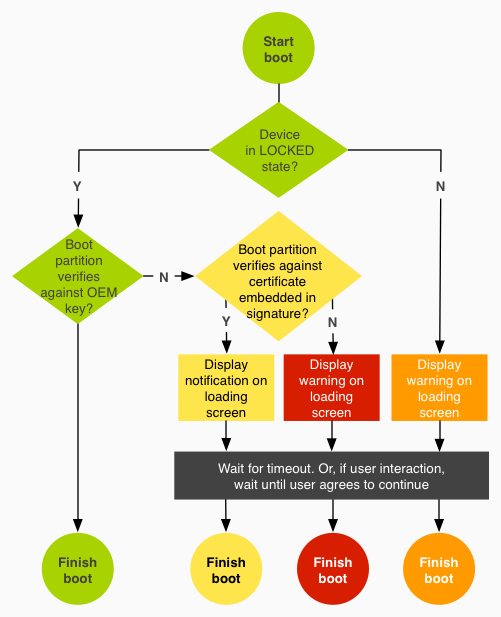
\includegraphics[width=0.55\linewidth]{chapter3/verified_boot}
		\caption{Diagrama de flujo del \textit{Arranque seguro} \cite{asreview2015}.}
		\label{fig:ch03:verifyBoot}
	\end{center}
\end{figure}
\subsection{Cifrado de la partición de datos}
Mediante una opción de la configuración, Android permite cifrar todos los datos de usuario presentes en un dispositivo, utilizando claves de cifrado simétricas. Una vez cifrado, el proceso es transparente para el usuario. Es decir, todos los datos creados se cifran antes de enviarlos al disco y todas las lecturas descifran los datos antes de devolverlos al proceso que realizó la llamada.\\

Esta funcionalidad se activa desde \texttt{Ajustes/Seguridad/Cifrar Teléfono}, como se observa en la Figura \ref{fig:ch03:android-cifrado}. Al activarse dicha opción, se cifran los datos privados de las aplicaciones, el contenido de la tarjeta SD y los datos personales, pudiendo cambiar más adelante el alcance de los componentes afectados por el cifrado. Mientras esté activa dicha opción, cada vez que arranque el dispositivo, el usuario debe proporcionar sus credenciales para poder acceder a cualquier parte del disco.\\
La primera vez que apareció esta funcionalidad fue en la versión 3.0. Sin embargo, a partir de la versión 5.0, fue fuertemente recomendado a los fabricantes de dispositivos que habiliten esta característica. La novedad incorporada en Android Marshmallow es que se puede cifrar el contenido de la tarjeta SD, permitiendo que sea ilegible si es removida del dispositivo.
\begin{figure}[htbp]
	\begin{center}
		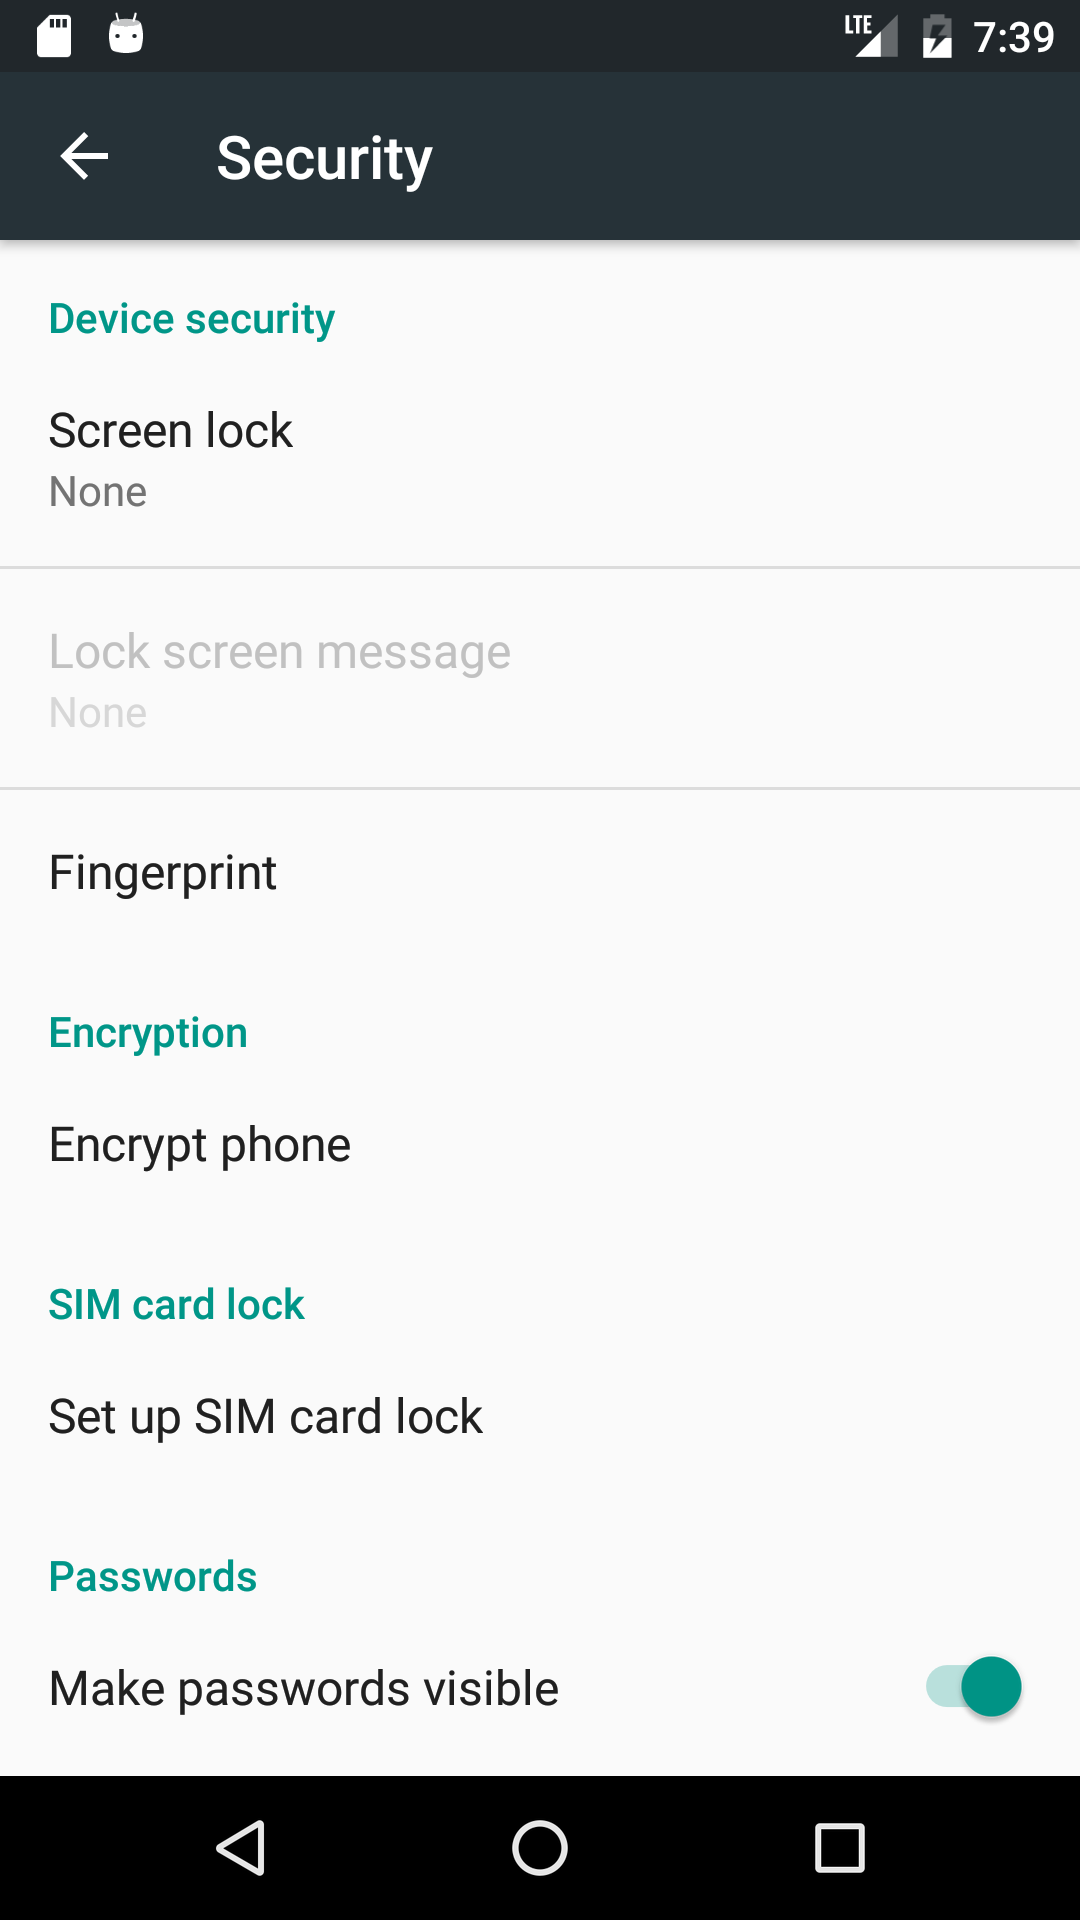
\includegraphics[width=0.3\linewidth]{chapter3/android-cifrado}
		\caption{Captura de \texttt{Ajustes/Seguridad}.}
		\label{fig:ch03:android-cifrado}
	\end{center}
\end{figure}
\subsection{Permisos}\label{ch03-permisos}
Debido a que cada aplicación Android opera en un \emph{entorno aislado}\footnote{Ver sección \nameref{ch01-sandbox}.}, las aplicaciones deben compartir de manera explícita recursos y datos. El camino utilizado para realizar dicho intercambio es la declaración de permisos, tal como se introdujo en la sección \ref{ch01-permisos}. El presente informe se centra en los permisos \emph{Normales} y \emph{Peligrosos}; cómo se otorgan y cómo se deniegan.\\

En las versiones anteriores a Android Marshmallow, al prepararse para instalar una aplicación, el sistema operativo mostraba un diálogo al usuario indicando los permisos solicitados y se le solicitaba si deseaba continuar con la instalación. En caso afirmativo, el sistema otorgaba todos los permisos solicitados e instalaba la aplicación. En el caso contrario, no se instalaba la aplicación. El usuario quedaba preso si quería instalar una aplicación: no podía otorgar o denegar permisos individuales; debía otorgar o denegar todos los permisos solicitados como un bloque. Una vez concedidos, los permisos seguían vigentes mientras la aplicación este instalada. Solo se eliminaban si se desinstala dicha aplicación.\\

A partir de la versión 6.0, se propone un nuevo modelo de permisos, donde los usuarios pueden administrar en tiempo de ejecución los permisos \emph{peligrosos} requeridos por una aplicación. En este modelo, los permisos se agrupan para facilitar el control de la privacidad de los usuarios.\\

Dichos grupos son:
\begin{itemize}
    \item \emph{Almacenamiento:} Regula el acceso al almacenamiento externo\footnote{En Android, cuando se habla de almacenamiento externo, se refiere a la tarjeta SD.}, \\permitiendo la lectura o la escritura desde el mismo.
    \item \emph{Calendario:} Permite leer, modificar o eliminar los calendarios del usuario. Incluye además el manejo de los eventos presentes en un calendario.
    \item \emph{Cámara:} Regula el acceso de la cámara del dispositivo, permitiendo capturar imágenes y grabar videos.
    \item \emph{Contactos:} Permite leer, modificar o eliminar los contactos presentes en el dispositivo.
    \item \emph{Localización:} Regula el acceso a la ubicación del dispositivo, ya sea la ubicación precisa (GPS) o la ubicación aproximada (WIFI/Móvil).
    \item \emph{Mensajes SMS:} Permite escribir mensajes SMS, leerlos o eliminarlos. Además, permite interceptar los mensajes entrantes.
    \item \emph{Micrófono:} Regula el acceso al micrófono del dispositivo, permitiendo además grabar el sonido obtenido. No se incluyen en este grupo los permisos para capturar sonidos provenientes de una llamada telefónica.
    \item \emph{Teléfono:} Regula el acceso a la información relacionada a una llamada telefónica, tales como iniciar una llamada, obtener datos de una llamada en curso, manipular el log de llamadas, entre otros.
    \item \emph{Sensores:} Permite acceder a los datos de los sensores del dispositivo. Se incluyen el giroscopio, el acelerómentro, sensor del ritmo cardíaco, entre otros.
\end{itemize}
En contraposición a lo que ocurría en las versiones previas, en Android Marsmallow durante la instalación de una aplicación se le otorgan todos los permisos \emph{normales} y ningún permiso \emph{peligroso}. Como consecuencia de esto, cada vez que una aplicación necesita acceder a un recurso protegido por un permiso \emph{peligroso}, tiene que solicitarlo en tiempo de ejecución. Por ejemplo, si una aplicación requiere leer un contacto, la primera vez aparece una notificación pidiendo autorización explicita al usuario, tal como se observa en la Figura \ref{fig:ch01:permission-request}. El usuario puede otorgar el permiso, denegarlo una vez o denegarlo para siempre. Si elige la última opción, no volverá a aparecer la notificación solicitando dicho permiso. Dichas opciones se encuentran en \texttt{Ajustes/Aplicaciones/\{nombre de la aplicación\}/Permisos}. En la Figura \ref{fig:ch03:app-permissions-overview} se observa una captura de las configuraciones de los permisos para una aplicación móvil.\\

Debido a que el usuario puede revocar algunos los permisos en cualquier momento, una aplicación debe comprobar si dispone de ellos cada vez que se ejecuta. De lo contrario no va a poder acceder a las funciones de las cuales no tiene permiso. Sin embargo, el usuario no puede revocar los permisos \emph{normales}; solamente se eliminan al desinstalar la aplicación.
\begin{figure}[btp]
    \centering
    \begin{subfigure}{0.35\linewidth}
        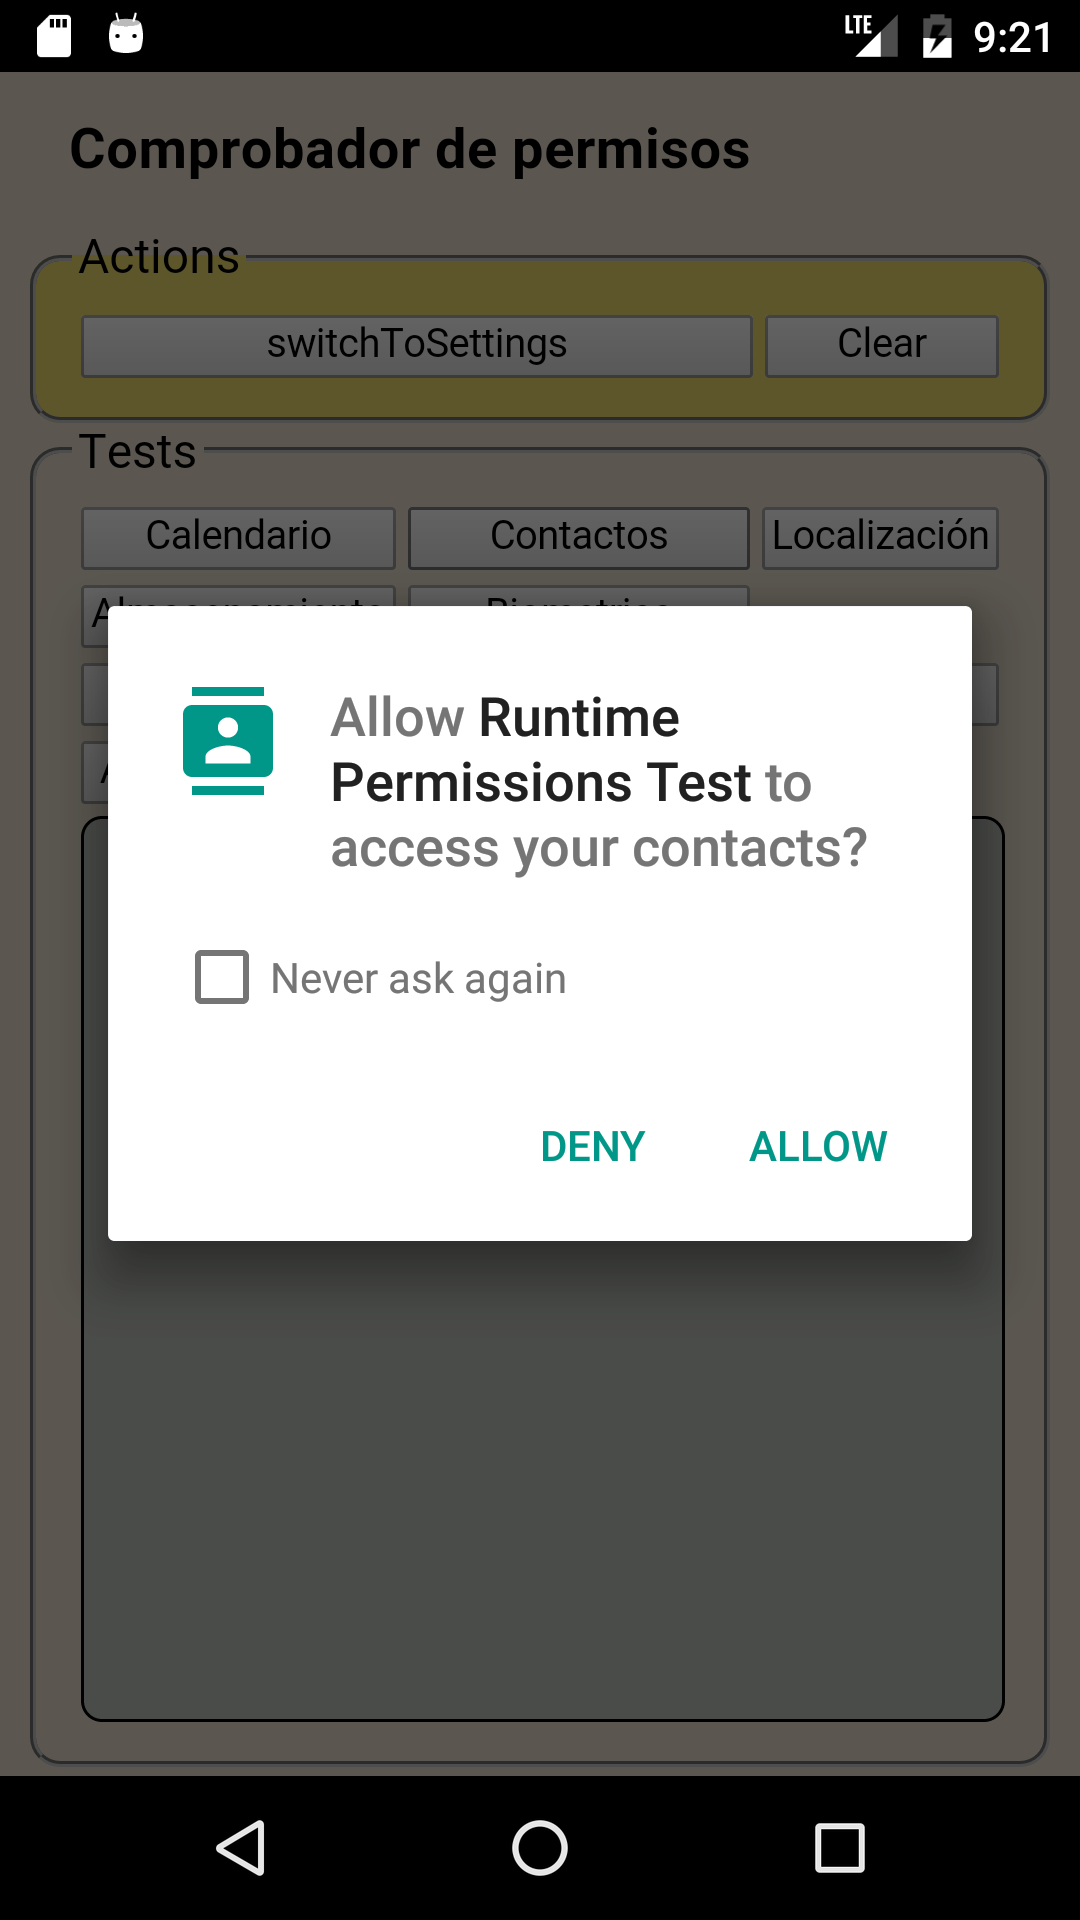
\includegraphics[width=\linewidth]{imgs/chapter5/allow_contact}
        \caption{Solicitud de un permiso en tiempo de ejecución.}
        \label{fig:ch01:permission-request}
    \end{subfigure}
    \begin{subfigure}{0.35\linewidth}
        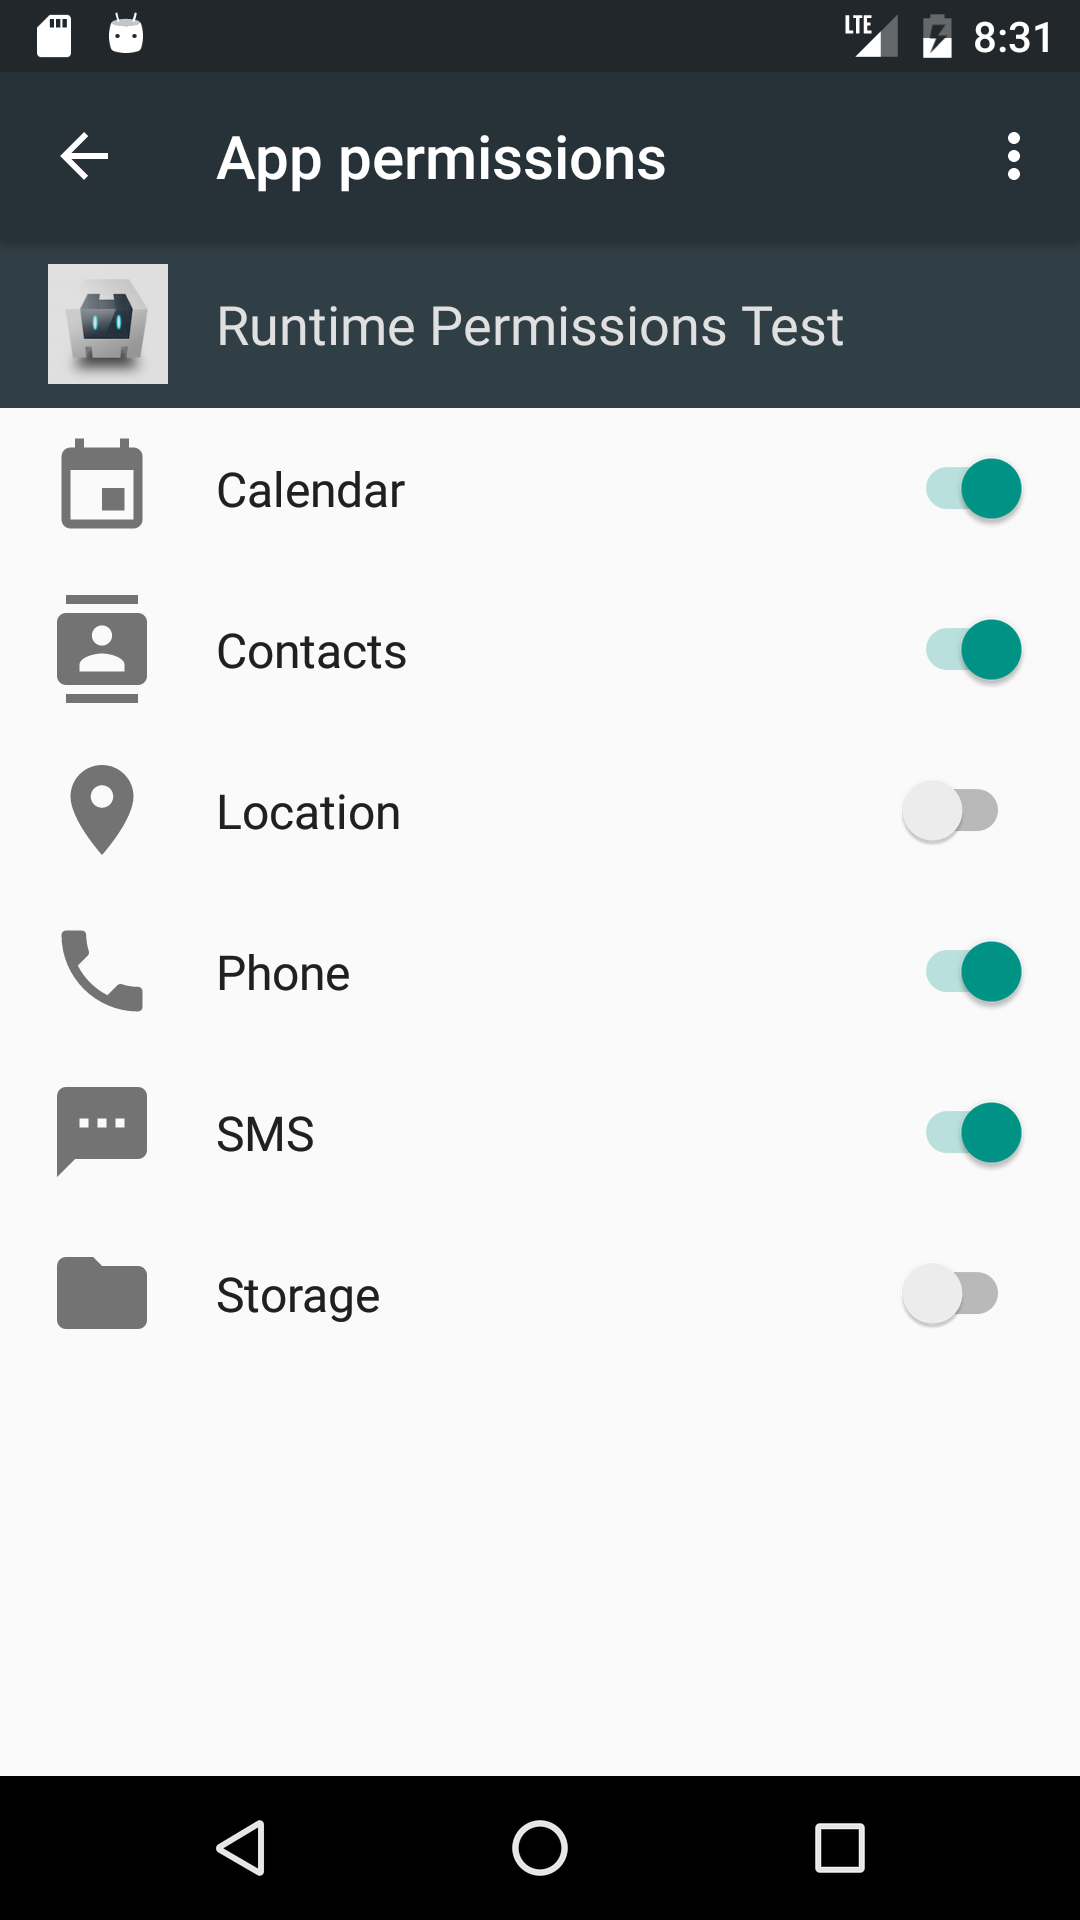
\includegraphics[width=\linewidth]{imgs/chapter1/app-permissions}
        \caption{Descripción general de los permisos otorgados.}
	    \label{fig:ch03:app-permissions-overview}
	\end{subfigure}
	\caption{Permisos en Android Marsmallow.}
	\label{fig:ch03:app-permissions-android}
\end{figure}
\section{Analizando iOS}
\subsection{Bloqueo del dispositivo}
Al configurar el código de desbloqueo para un dispositivo, el usuario activa la protección de datos automáticamente. El sistema admite códigos alfanuméricos de cuatro dígitos, de seis dígitos y de longitud arbitraria, salvo que el dispositivo tenga un lector de huellas; en ese último caso deberá contar con al menos seis dígitos.\\

Además de desbloquear el dispositivo, el código provee entropía a ciertas claves de cifrado del sistema. El hecho de que esté muy ligado con el UID, añade una seguridad extra: no se puede intentar quebrar dicho código fuera del dispositivo. Es por ello que cuanto más seguro sea el código de desbloqueo, más segura será la clave de cifrado.\\

A fin de desalentar los posibles ataques de fuerza bruta, se generan retardos cada vez mayores tras la introducción de un código inválido en la pantalla de bloqueo. Los retardos están calibrados suponiendo que la frecuencia entre un ataque y otro es de 80 milisegundos \cite{asg}. En dispositivos que cuentan con un \textit{Secure Enclave}, los retardos se aplican mediante dicho componente. Si el dispositivo se reinicia durante un tiempo de demora, la demora aún se aplica, con el temporizador empezando de nuevo para el periodo actual.
\subsection{Arranque seguro}\label{fig:ch02:arranque}
Cada dispositivo es seguro desde el arranque, ya que la arquitectura del sistema fue pensada para integrar \textit{hardware}, \textit{software} y servicios, con el objetivo de obtener seguridad a lo largo de todos los componentes que conforman el núcleo del sistema \cite{asg}. Cuando se prende un dispositivo cuyo sistema operativo es iOS, se siguen los siguientes pasos para asegurar la integridad del arranque del sistema\footnote{Traducción propuesta para el término \textit{Boot Chain}} :
\begin{enumerate}
	\item Se ejecuta el código alojado en la \textit{BootROM}. Dicho código es inmutable y seguro por definición.
	\item Se verifica la firma del \textit{bootloader} LLB\footnote{\textit{Low Level Bootloader}, por sus siglas en inglés}, ya que fue certificado por Apple con la clave pública \textit{Apple Root CA}. La misma está alojada en la \textit{BootROM}. 
	\item Pasada la validación, empieza la carga del kernel de iOS mediante \textit{iBoot}.
	\item El siguiente paso es asegurar la integridad del software. Los dispositivos con un procesador A7 o superior, cuentan con un coprocesador llamado \textit{Secure Enclave}\footnote{\textit{Secure Enclave} es un coprocesador con memoria cifrada e incluye generación de números aleatorios por hardware \cite{asg}.} para verificar dicha integridad.
\end{enumerate}
Si fallan alguno de estos pasos, el dispositivo entra en \emph{Modo de Recuperación}\footnote{Traducción del término \textit{recovery mode}.} y se lo debe conectar a iTunes via USB para restaurar la configuración de fábrica.
\subsection{Cifrado de archivos}
Cada vez que se guarda un archivo en la partición de datos, el sistema operativo crea una clave AES-256 para ése archivo. Dicha clave es única y es utilizada por el \textit{Secure Enclave} para cifrar el archivo. Luego, ésa clave se empaqueta con una (o varias) de las claves de clases, dependiendo de la accesibilidad que va a tener el archivo \cite{asg}.\\

Cada vez que se abre un archivo, ocurre el proceso inverso: su metadata es desempaquetada con la clave del sistema de archivos, revelando la clave particular del archivo y las clases que lo protegen. Se vuelve a desempaquetar, esta vez, con las claves de las clases, para finalmente descifrar al archivo con su clave única. El proceso completo se observa en la Figura \ref{fig:ch02:dataProtection}.
\begin{figure}[hbtp]
    \centering
    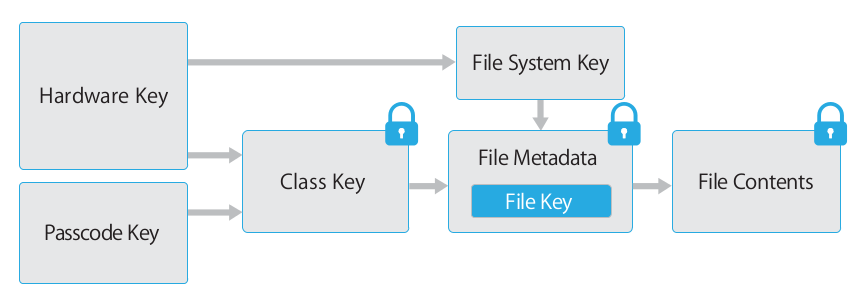
\includegraphics[width=.7\linewidth]{chapter2/ios_fileDataProtection_architecture}
    \caption{Proceso para descifrar un archivo \cite{asg}.}
    \label{fig:ch02:dataProtection}
\end{figure}
\subsection{Firma de código de las aplicaciones}
iOS garantiza que todas las aplicaciones proceden de una fuente conocida y aprobada. Por ello, requiere que todo el código ejecutable se firme con un certificado emitido por Apple. La firma de código obligatoria extiende el concepto de cadena de confianza del sistema operativo a las aplicaciones e impide que aplicaciones de terceros carguen código sin firmar o utilicen código que se modifique automáticamente.\\

Para poder desarrollar aplicaciones en dispositivos iOS, los desarrolladores deben registrarse. Apple verifica la identidad real de cada desarrollador, ya sea una persona individual o una empresa, antes de emitir su certificado. Este certificado permite a los desarrolladores firmar sus aplicaciones y enviarlas a la tienda para su distribución. Además, todas las aplicaciones de la tienda han sido revisadas para garantizar que funcionan según lo esperado y que no contienen errores ni otros problemas evidentes.\\

A diferencia de otras plataformas móviles, iOS no permite a los usuarios instalar aplicaciones procedentes de sitios web que no estén firmadas, ni ejecutar código que no sea de confianza \cite{asg}. Durante la ejecución de una aplicación, se comprueba la firma de código de todas las páginas de la memoria ejecutable a medida que se cargan para garantizar que una aplicaciones no se ha modificado desde la última vez que se instaló o actualizó \cite{asg}.
\subsection{Permisos}
Los controles de privacidad en iOS restringen el acceso de las aplicaciones a la información personal del usuario. El principal control es el sistema de permisos, el cual es encargado de custodiar el acceso a ciertos recursos. Al momento de instalar una aplicación en el dispositivo, no le se otorga ningún permiso. Es responsabilidad de cada aplicación solicitar los permisos que requiere al momento de utilizar el recurso custodiado. Por ejemplo, en la Figura \ref{fig:chapter03:iospermCapture} se observa el pedido del permiso al componente Calendario. Sin la autorización explícita del usuario, dicha aplicación tiene restringido el acceso a ese recurso.\\

\begin{figure}[hbtp]
	\centering
	\begin{subfigure}{.33\linewidth}
    	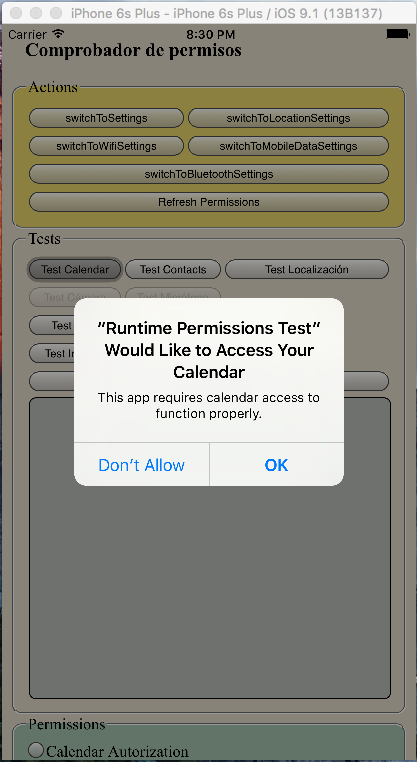
\includegraphics[width=\linewidth]{chapter3/calendar_request_ios}
	    \caption{Captura del pedido de un permiso.}    		
	    \label{fig:chapter03:iospermCapture}
    \end{subfigure}
    \begin{subfigure}{.33\linewidth}
    	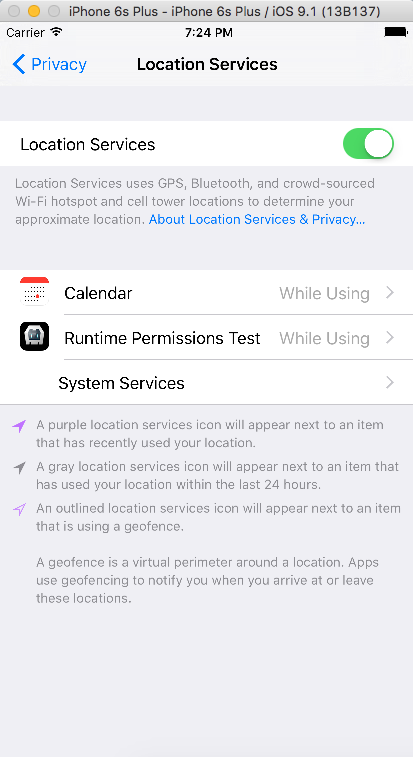
\includegraphics[width=\linewidth]{chapter3/apps-allow-location}
	    \caption{Aplicaciones que requirieron un permiso.}    		
	    \label{fig:chapter03:privacy}
	\end{subfigure}
	\caption{Permisos en iOS 9.}    		
	\label{fig:chapter03:app-permissions-ios}
\end{figure}
\newpage
El usuario puede modificar la configuración de privacidad desde \texttt{Ajustes/Privacidad}. Se pueden aprobar o denegar cualquier permiso que haya sido solicitado. Aún más, se puede denegar ``para siempre'': está pensado para evitar que aparezca constantemente una notificación solicitando determinado permiso. En la Figura \ref{fig:chapter03:privacy} se observan las aplicaciones que requirieron el permiso \emph{Localización}.\\

Los permisos restringen el acceso a:
\begin{itemize}
	\item \emph{Localización:} Permite determinar aproximadamente la ubicación del dispositivo. Utiliza una combinación de cierta información del celular, WiFi, Bluetooth y GPS para determinarla.
	\item \emph{Contactos:} Regula el acceso a los contactos del dispositivo, ya sea para crearlos, modificarlos o eliminarlos.
	\item \emph{Calendarios:} Regula el acceso a los calendarios, incluyendo las citas y eventos incluidos en él.
	\item \emph{Recordatorios:} Permite leer, modificar o eliminar un recordatorio. Los recordatorios son pequeñas notas, listas de tareas, entre otras cosas.
	\item \emph{Fotos:} Regula el acceso a la galería de imágenes de la cámara. También tiene la capacidad de crear un álbum de fotos dentro de la aplicación de fotos.
	\item \emph{Compartir a través de Bluetooth:} Regula cuáles aplicaciones pueden compartir datos a través de Bluetooth.
	\item \emph{Micrófono:} Regula el acceso al micrófono.
	\item \emph{Cámara:} Regula el acceso al la cámara del dispositivo.
	\item \emph{Salud:} Regula el acceso a la información de salud y estado físico del usuario, tanto las que recopiló el dispositivo como las insertadas por el usuario.
	\item \emph{HomeKit:} Regula el acceso a los accesorios hogareños registrados en el dispositivo.			
	\item \emph{Redes Sociales:} Permite realizar actividades relacionadas a una red social, tales como crear una sesión de red, obtener el feed de actividad para un usuario, hacer una nueva entrada.
	\item \emph{Diagnóstico:} Regula cuáles datos de diagnóstico sobre el dispositivo se envían a Apple. Esos datos incluyen información sobre el rendimiento del sistema, capacidad restante en el dispositivo, entre otras.
	\item \emph{Publicidad:} Permite inhabilitar los anuncios basados en intereses.
\end{itemize}
\section{Crítica}
Teniendo presente el análisis realizado en las secciones anteriores, se realiza a continuación una crítica sobre los modelos de seguridad de ambas plataformas. La misma está compuesta por cuatro niveles gradualmente más complejos que engloban aspectos de la seguridad que van desde que se prende el dispositivo hasta el uso de una aplicación.
\subsection{Arranque verificado}
Desde la primera versión, iOS ofrece la funcionalidad de verificación desde el arranque del dispositivo para ver si fue modificado respecto de la version de fábrica. Por lo tanto, dicha verificación es transparente para el usuario. En caso de fallar, el dispositivo entra en \emph{modo de recuperación}, teniendo que conectarlo a una computadora para restaurar la configuración de fábrica.\\

En Android, el arranque verificado se agregó en la version 4.4 pero recién en la versión 6.0 se hizo obligatorio para los fabricantes. La principal ventaja respecto de iOS es que tiene cuatro estados finales de la verificación en vez de dos. Se identifican por colores: verde, amarillo, naranja y rojo. Los estados verde y rojo son equivalentes a los estados de iOS: válido e inválido, respectivamente. Los estados amarillo y naranja corresponden a una validación parcial\footnote{Ver apartado \ref{fig:ch03:verify-boot}.}. Android deja librado a la decisión del usuario para continuar o suspender el arranque.
\subsection{Cifrado del sistema de archivos}
Tanto Android con iOS proveen la funcionalidad de cifrar los datos alojados en el sistema de archivos. Sin embargo, tienen una política distinta al momento de aplicarlo: en iOS está siempre habilitada y no se puede deshabilitar; mientras que en Android, se deja esta decisión al usuario.\\

En Android, al soportar almacenamiento externo, se corre el riego de que se accedan a los datos por fuera del dispositivo. Es por ello que, a partir de la versión 6.0, el usuario puede cifrar la tarjeta SD. De esta manera, reduce el riesgo mencionado.\\

Por su parte, iOS está libre del riesgo mencionado en el párrafo anterior, ya que todo su almacenamiento es interno. Además, iOS agrega una medida extra de seguridad: los archivos se cifran utilizando varias claves, entre las que se encuentran el código de desbloqueo y UID\footnote{Clave única por dispositivo. Más datos en la sección \ref{fig:ch02:data-protection}.}. Gracias a ello, se dificulta muchísimo la tarea de quebrar el cifrado por fuera del dispositivo.
\subsection{Bloqueo del dispositivo}
Android cuenta con cinco métodos de bloqueo de pantalla: PIN, patrón, contraseña, desbloqueo facial y huella digital. Por otro lado, iOS dispone de sólo dos métodos: PIN y huella digital.\\

Independientemente del método utilizado para bloquear la pantalla, tanto en Android como en iOS, el proceso de desbloqueo ocurre en un entorno seguro (TEE y \emph{Secure Enclave}, respectivamente). Como consecuencia de esto, las claves se procesan siempre allí y no son conocidas por el resto de los componentes. Además, se incrementa el tiempo de espera del bloqueo, dificultando un ataque por fuerza bruta.\\

iOS agrega una medida de seguridad extra: el código de desbloqueo está muy ligado al UID. Es por ello que no se puede realizar ataques al código de desbloqueo fuera del dispositivo.
\subsection{Seguridad de las aplicaciones}
Inicialmente, tanto Android como iOS tienen un enfoque similar, en el sentido de que ambos se apoyan en sus propias tiendas de aplicaciones en los que comprueban la seguridad de las miles de aplicaciones que se encuentran a disposición del usuario. Sin embargo, tienen una diferencia filosófica respecto de los proveedores de aplicaciones: en iOS todas las aplicaciones tienen que descargarse de la tienda oficial. Es más, para poder subir una aplicación, su desarrollador pasa por un proceso muy estricto de registro. En cambio, al ser un sistema más abierto, Android favorece la instalación de aplicaciones de terceros, ya que deja abierta la posibilidad de instalar aplicaciones ``sueltas'' e incluso tiendas. Es peligroso, pero le da una flexibilidad inmensa, frente a la rigidez de iOS. Esta libertad, sin embargo, tiene un precio, y es la presencia de \emph{malware} disfrazado de aplicaciones legítimas.\\

Respecto a la ejecución de una aplicación, Ambos sistemas aislan los procesos en ejecución en un \emph{entorno aislado}\footnote{Traducción propuesta para el término \textit{sandbox}.}. Como consecuencia de esto, se destacan dos resultados: evita que una aplicación pueda tomar control de todo el sistema; y evita que una aplicación conozca datos de otra.\\

Al comparar la gestión de permisos de ambas plataformas, encontramos varias similitudes. Lo primera cosa en común es que a las aplicaciones no se le otorgan ningún permiso al momento de instalarla. Otra cosa que comparten es que si una aplicación necesita algún permiso, debe requerirlo mientras se ejecuta, pudiendo el usuario otorgar o denegarlo. La última similitud es que, desde la configuración de privacidad, el usuario puede revocar u otorgar permisos a las aplicaciones.\\

Respecto a cómo se definen los permisos, se observan diferencias de concepto. En Android están orientados según el riesgo implícito al otorgarlos. En cambio, en iOS, los permisos están orientados a los componentes. Sin embargo, se pueden comparar según los componentes que son afectados por un permiso. De esta manera, se puede saber cuáles componentes son protegidos por permisos en ambas plataformas y cuáles están presentes solamente en una de ellas. Con estos datos, se confeccionó la Tabla \ref{tab:chapter03:compPerm}.\\

\begin{table}[tbp]
	\center
	\begin{tabular}{c c c}
		\hline
		\multicolumn{3}{c}{\textbf{Permisos}} \\
		\emph{Ambas plataformas} 	& \emph{Solo en Android}	& \emph{Solo en iOS} \\ \hline    \hline
		Calendario	& -		& -	\\						
		Contactos	& -				& - \\						
		Cámara		& -				& -	\\						
		Localización& -				& -	\\						
		-			& -				& Compartir por Bluetooth\\ 
		Micrófono   & -				& - \\						
		-			& Teléfono		& -	\\						
		Sensores    & -    			& - \\						
		-			& SMS			& - \\						
		-			& Almacenamiento& - \\						
		-			& -				& \emph{Homekit} \\			
		-			& -				& Redes Sociales \\        	
		-			& -				& Diagnóstico \\        			
		-			& -				& Publicidad \\    			\hline
	\end{tabular}
	\caption{Comparación de permisos entre Android 6.0 e iOS}
	\label{tab:chapter03:compPerm}
\end{table}
Respecto del alcance del sistema de permisos, se observó una falta de granularidad de los permisos que se pueden modificar \emph{en tiempo de ejecución}. En Android, un permiso es a nivel de grupo. Por lo tanto, el usuario otorga o deniega para todo el grupo. Por ejemplo, si se pide permisos del grupo \emph{Contactos} se obtienen los permisos para leer, modificar o eliminar los contactos. Para  una aplicación que administra los contactos tiene sentido tener todos los permisos, pero para una aplicación de acceso a una red social, no tiene sentido que pueda eliminar un contacto. La misma situación ocurre en iOS: se otorga un permiso de acceso a todas las funcionalidades de un determinado componente. Como consecuencia de ello, el usuario esta delegando a una aplicación demasiados permisos y no tiene expresividad para decir que funcionalidades autoriza.\\

Otra cosa a destacar es la cobertura del sistema de permisos. Las dos plataformas dejan funcionalidades principales del dispositivo sin permisos modificables \emph{en tiempo de ejecución}. En Android, los permisos \emph{normales} son otorgados al instalarse la aplicación y no pueden ser quitados. Entre ellos se encuentran: Acceso a Internet, Compartir vía Bluetooth, Información del dispositivo, entre otros. Además, no hay un permiso para proteger los datos de las Redes Sociales. Por su parte, iOS también deja algunos componentes sin permisos modificables \emph{en tiempo de ejecución}. Entre ellos se encuentran: Acceso a Internet, SMS, entre otros. Tampoco tiene la suficiente granularidad para administrar el acceso a los datos de las llamadas telefónicas.\\

Para finalizar se hablará sobre como se muestra al usuario los permisos adquiridos por una aplicación. En iOS solamente se listan los permisos requeridos por una aplicación, como se observa en la Figura \ref{fig:ch05:ios_all_permissions}. En cambio, en Android es confuso como se informa. En la Figura \ref{fig:ch05:without_permissions} se observa las datos de una aplicación. Si se observa el apartado \emph{Permisos}, la leyenda indica que no fueron otorgados ningún permiso \emph{peligroso}. Ingresando en ese apartado, queda claro lo mencionado anteriormente. Sin embargo, dada dice sobre los demás permisos. Si se presiona sobre los tres puntos, se acceden a todos los permisos, como se observa en la Figura \ref{fig:ch05:always_have_internet}. Ahí nace la confusión: primero indica que ``No hay permisos otorgados'', pero indagando un poco, se descubre que fueron otorgados todos los permisos \emph{normales}.
\begin{figure}[hbtp]
	\centering
	\begin{subfigure}{.3\linewidth}
		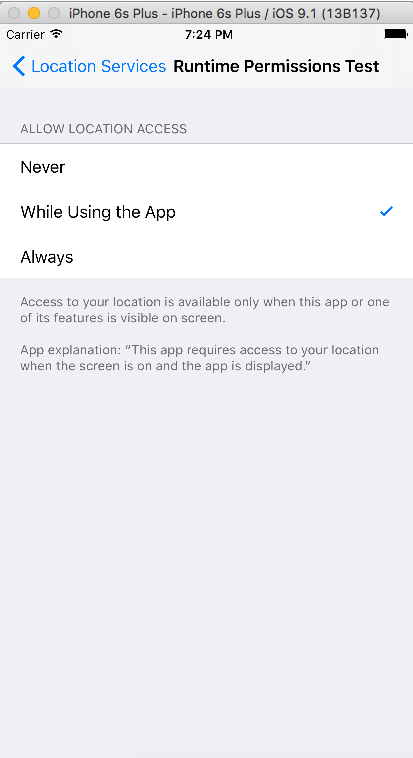
\includegraphics[width=\linewidth]{chapter2/permission-classes.png}
		\caption{Permisos requeridos por una aplicación.}
		\label{fig:ch05:ios_all_permissions}
	\end{subfigure}
	\begin{subfigure}{.3\linewidth}
		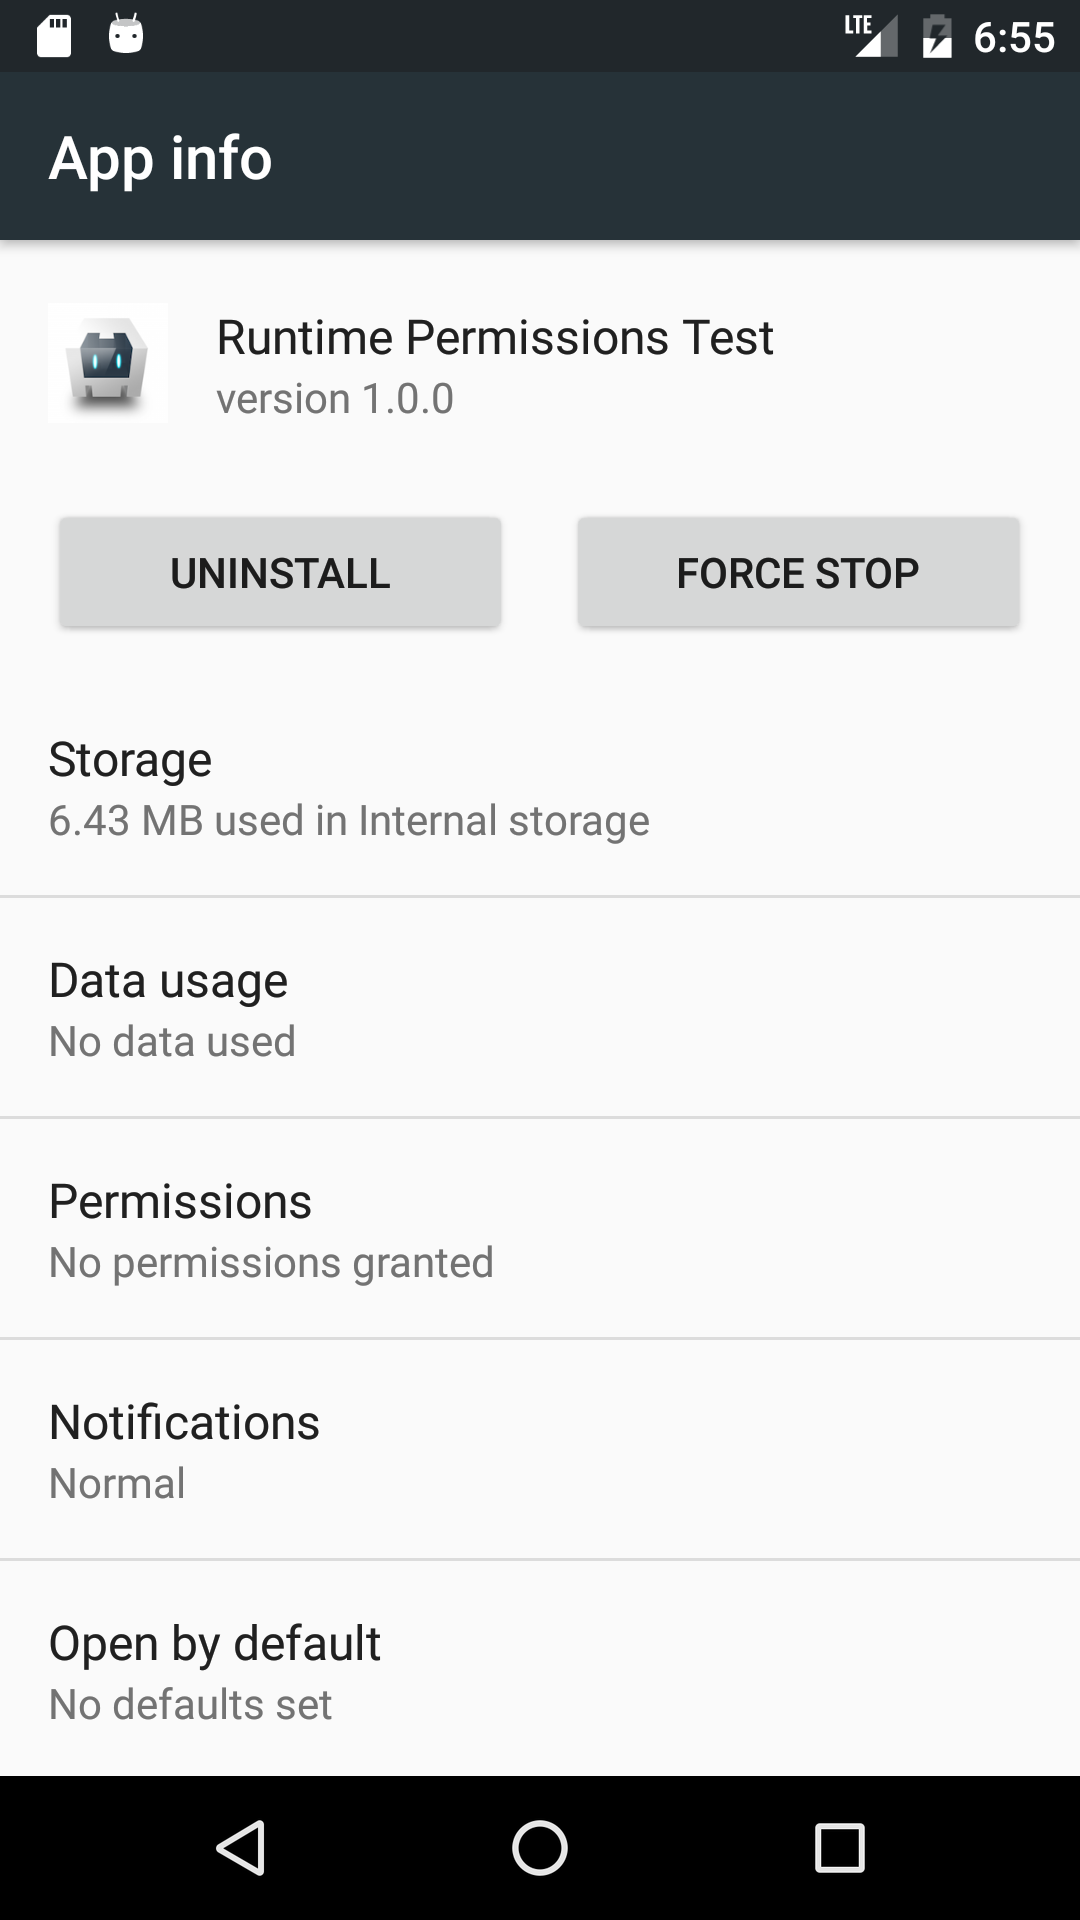
\includegraphics[width=\linewidth]{chapter5/no_permissions_granted}
		\caption{La aplicación no tiene ningún permiso.}
		\label{fig:ch05:without_permissions}
	\end{subfigure}
	\begin{subfigure}{.3\linewidth}
		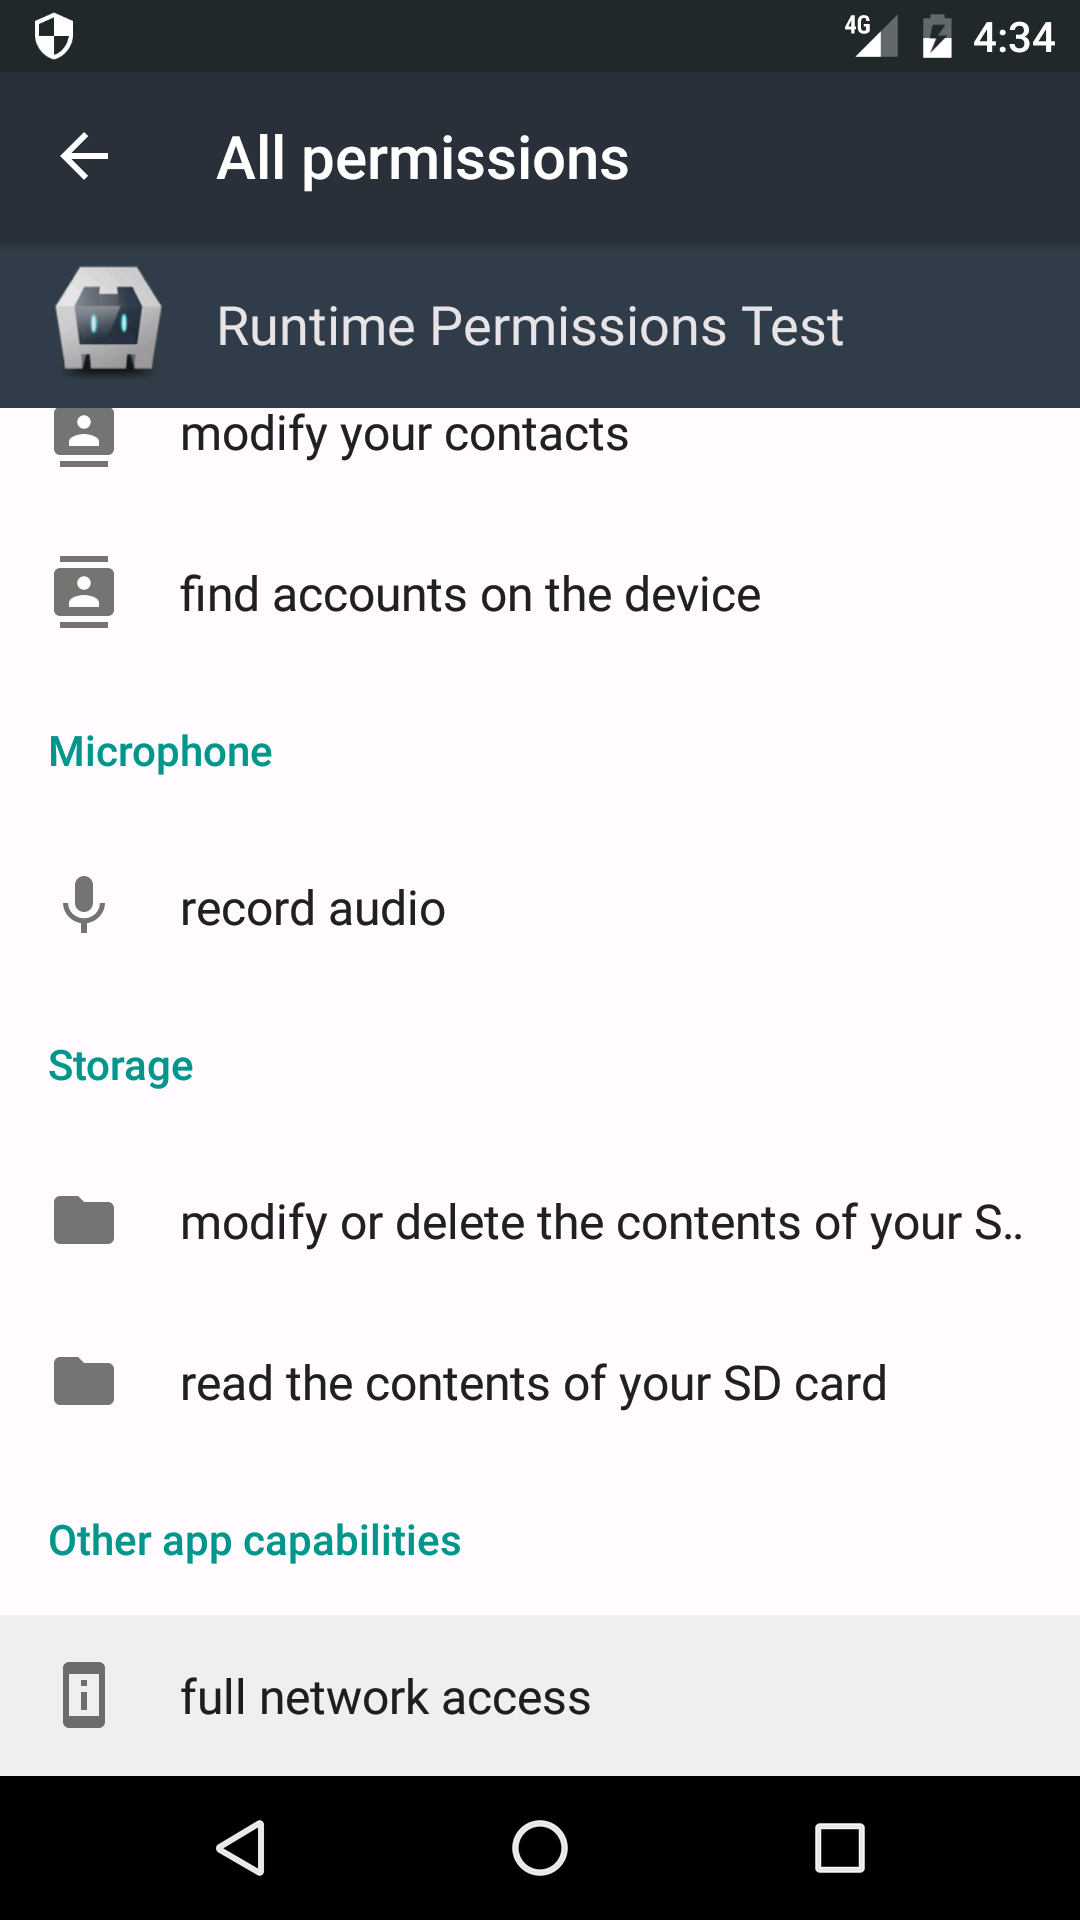
\includegraphics[width=\linewidth]{chapter5/always_have_internet}
		\caption{Tiene todos los permisos \emph{normales}.}
		\label{fig:ch05:always_have_internet}
	\end{subfigure}
\end{figure}